\documentclass{acm_proc_article-sp}
\usepackage{hyperref}
\usepackage{graphicx}
\usepackage{listings}
\usepackage{paralist}
\usepackage{xcolor}
\colorlet{punct}{red!60!black}
\definecolor{background}{HTML}{EEEEEE}
\definecolor{delim}{RGB}{20,105,176}
\colorlet{numb}{magenta!60!black}

\lstdefinelanguage{json}{
    basicstyle=\scriptsize\ttfamily,
    numbers=left,
    numberstyle=\scriptsize,
    stepnumber=1,
    numbersep=7pt,
    showstringspaces=false,
    breaklines=true,
    frame=lines,
    backgroundcolor=\color{background},
    literate=
     *{0}{{{\color{numb}0}}}{1}
      {1}{{{\color{numb}1}}}{1}
      {2}{{{\color{numb}2}}}{1}
      {3}{{{\color{numb}3}}}{1}
      {4}{{{\color{numb}4}}}{1}
      {5}{{{\color{numb}5}}}{1}
      {6}{{{\color{numb}6}}}{1}
      {7}{{{\color{numb}7}}}{1}
      {8}{{{\color{numb}8}}}{1}
      {9}{{{\color{numb}9}}}{1}
      {:}{{{\color{punct}{:}}}}{1}
      {,}{{{\color{punct}{,}}}}{1}
      {\{}{{{\color{delim}{\{}}}}{1}
      {\}}{{{\color{delim}{\}}}}}{1}
      {[}{{{\color{delim}{[}}}}{1}
      {]}{{{\color{delim}{]}}}}{1},
}

\renewcommand{\lstlistingname}{Code}

\begin{document}

\title{Adaptive Linked Data-driven Web Components:\\ Building Flexible and Reusable Semantic Web Interfaces}
\subtitle{}

\numberofauthors{3} %  in this sample file, there are a *total*
\author{
% 1st. author
\alignauthor
Ali Khalili\\
       \affaddr{Dept. of Computer Science}\\
       \affaddr{VU University Amsterdam}\\
       \affaddr{The Netherlands}\\
       \email{a.khalili@vu.nl}
% 2nd. author
\alignauthor
Antonis Loizou\\
       \affaddr{Dept. of Computer Science}\\
       \affaddr{VU University Amsterdam}\\
       \affaddr{The Netherlands}\\
       \email{a.loizou@vu.nl}
% 3rd. author
\alignauthor
Frank van Harmelen\\
       \affaddr{Dept. of Computer Science}\\
       \affaddr{VU University Amsterdam}\\
       \affaddr{The Netherlands}\\
       \email{frank.van.harmelen@vu.nl}
}


\maketitle
\begin{abstract}
% need to update the abstract
The amount of published Linked Data on the Web is increasing day by day.
As a result, the applications driven by Semantic Web and Linked Data are taking momentum on the Web.
One of the major entrance barriers for Web developers to contribute to this wave of Linked Data Applications (LDAs) is the required knowledge of Semantic Web technologies such as RDF data model and SPARQL query language to interact with the triple stores.
This paper presents an adaptive component-based approach together with its open source implementation for creating flexible and resuable Semantic Web interfaces driven by Linked Data.
Linked Data-driven (LD-R) Web components abstract the complexity of underlying Semantic Web technologies in order to allow reuse of existing Web components in LDAs and to enable Web developers who are not expert in Semantic Web to develop interfaces to view, edit and browse Linked Data.
In addition to modularity provided by the LD-R components, the proposed RDF-based configuration method allows application assemblers to reshape their user interface for different use cases, by either reusing existing shared configurations or by creating their proprietary configurations.

\end{abstract}


% % A category with the (minimum) three required fields

\category{D.2.13}{Software Engineering}{Reusable Software}

\terms{Design, Human Factors, Standardization}

%\keywords{
%Linked Data, refinement operators, data cleansing, RDF transformation
%} % NOT required for Proceedings

\section{Introduction}

%\begin{center}
%``The measure of intelligence is the ability to change.''  Albert Einstein
%\end{center}

With the growing number of structured data published on the Web, WWW is moving towards becoming a rich ecosystem of machine-understandable Linked Data (LD)~\footnote{\url{lodlaundromat.org} recently (25.09.2015) reported approx. 38.6 billion triples published on the Web.}.
Semantically structured data facilitate a number of important aspects of
information management such as information retrieval, search, visualization,  customization, personalization and integration~\cite{SCAJ-Khalili-2013}.
Despite all these benefits, Linked Data Applications (LDAs) have not yet grasped well by the large community of Web developers outside the Semantic Web domain and causally, by the end users on the Web.
%can we add some evidence?
The usage of semantic data is still quite limited and most of the currently published Linked Data are generated by a relatively small amount of publishers~\cite{ontowiki-swj} which indicate some entrance barriers towards wide-spread utilization of Linked Data~\cite{StegemannZ14}.

%describe issues
The current communication gap between Semantic Web developers and User Experience (UX) designers, driven by the need to bear Semantic Web knowledge, prevents streamline flow of best practices from UX community into the Linked Data user interfaces (UIs).
The resulting lack of adoption and standardization makes current LDAs not often function consistent with user expectations and impels more development time and costs on LDA deveopers.
In this situation, more time is spent in re-designing existing UIs rather than focusing on innovation and creation of sophisticated LDAs.
 
This paper presents adaptive Linked Data-driven Web components as an approach to build flexible and reusable Semantic Web UIs.
\emph{Web Components} are a set of W3C standards~\cite{webcomponentsW3C} that enable the creation of reusable widgets or components in Web documents and Web applications.
Resource Description Framework (RDF), on the other hand, provides a common data model that allows data-driven components to be created, shared and integrated in a structured way across different applications.
Linked Data-driven (LD-R) Web components as defiend in this paper are a species of Web components that employ RDF data model for representing their content and specification (i.e. metadata about the component).
LD-R components are supported by a set of predefined core Web components each representing a compartment of the RDF data model on the Web UI.
LD-R components enable encapsualtion of the Semantic Web nature of an LDA thereby allow UX designers and Web developers outside the Semantic Web community to contribute to LDAs.
They also allow current Semantic Web developers to reuse existing Web components in their LDAs.
Furthermore, LD-R components exploit the power and flexibility of RDF data model in describing and sharing resources to provide a mechanism to adapt the Web interfaces based on the meaning of data and user-defined rules. 
%The RDF (Resource Description Framework) as the basic building block of the Semantic Web provides a general framework to describe resources on the Web.

LD-R approach offers many benefits that we will describe in the remainder of the paper. Among them are:

\paragraph{Bootstrapping LDA UIs} 
LD-R components exploit best practices from modern Web application development to bring an exhaustive architecture to perform separation of concerns and thereby bootstrapping an LDA by only selecting a minimal relavant configuration.
For example, a developer only needs to set the URL of his in-use SPARQL endpoint and start developing the viewer components without dealing with the underlying connection adapters and data flow mediators in the system.

\paragraph{Standardization and Reusability of LDA UIs} 
Instead of creating an LDA UI from the scratch, in the component-based development of LDA UIs, application assemblers choose from a set of standard UIs which will reduce the time and costs associated with creation of LDAs.
For example, to render DBpedia resources of type 'Location', a standard map can be reused.

\paragraph{Customization and Personalization of LDA UIs} 
RDF-based nature of LD-R components allow application assemblers to reshape their user interface based on the meaning of data or user context.
For example, for all the resources of type 'foaf:Person', the content can be rendered with a 'ContactCard' component.

\paragraph{Adoption of LDA UIs by non-Semantic Web developers and end-users} 
Abstracting the complexity of RDF and graph-based data representation, provides more \emph{Affordances}~\cite{Norman2013} for non-Semantic Web users to contribute to Linked Data UIs.
Engaging more UX designers and Web developers into LDA UIs will also result in more affordances on the end-user's side to better understand the possible actions and advantages of the LDAs.

\section{Contributions and Outline}
The contributions of this work are the concept of \emph{Adaptive LD-R Web components} and an open source implementation of it available at \url{http://ld-r.org}.
Our primary claim is that adopting a component-based approach that encapsualtes the main concerns of a Semantic Web application, paves the way to reuse existing best practices from the UX community within the LDAs hence building more usable and pervasive LDAs.

We explore this claim in stages.
First, we collect some data about the current status of Semantic Web UI development.
Next, we demonstrate how adaptive LD-R Web components can address the current issues in LDA UI development.
Finally, we discuss the implementation of our idea and its usage in real-world scenarios.

\begin{figure*}[tb]
  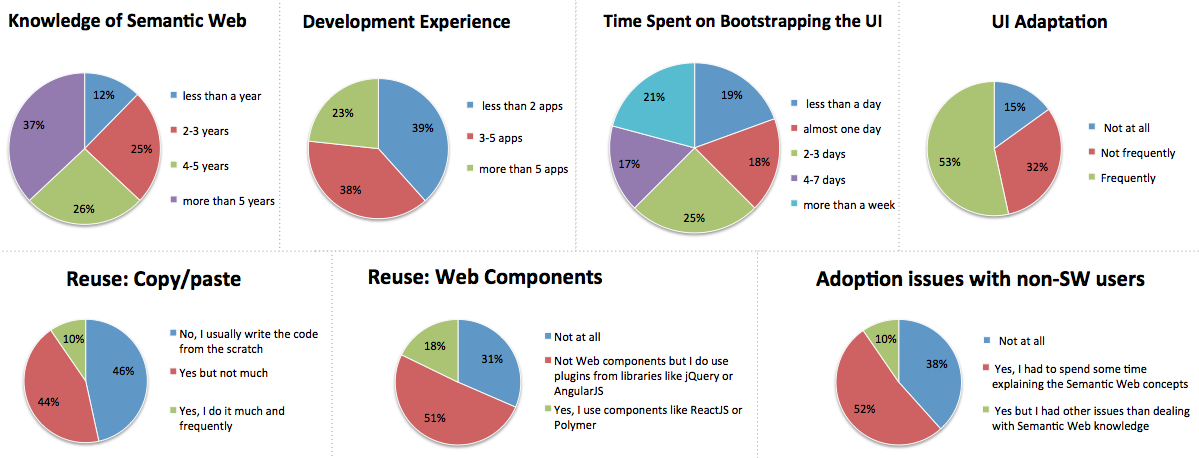
\includegraphics[width=1\linewidth]{images/userstudy.png}
  \caption{Results of our user study on the current status of LDA UI development.}
  \label{fig:userstudy}
\end{figure*}

\section{The Current Status of Linked Data User Interface Development}
In order to understand the current pitfalls of LDA UI design, we conducted a survey targeting \textbf{73} active Semantic Web developers~\footnote{results are available at \url{https://goo.gl/cltqhv}}.
The participants where selected from the community of Semantic Web developers on Github who have had at least one active Semantic Web-related repository.
We used Github APIs~\footnote{\url{https://developer.github.com/v3/}} to search~\footnote{keywords: "Semantic Web" OR "Linked Data" OR "RDF" OR "SPARQL"} for the potential Semantic Web repositories and then to collect the contact information of the corresponding contributors when available.
The search, after removing the organizations and invalid email addresses, resulted in 650 potential Semantic Web developers.
We then contacted the potential candidates to ask them about the current pitfalls in developing LDA UIs.
In our enquiry, we clearly mentioned to skip the questionnaire if they have not developed any Semantic Web application so far.
We used a set of 7 minimal viable questions to attract more people and also used inline forms for GMail users to allow filling out the questionnaire in the same time that reading the enquiry email.
The number of participants who filled in our questionnaire at the end was 73 (almost 11\% of the potential candidates which is still a considerable number of participants).
Questions addressed the following topics:

\paragraph{Knowldge of Semantic Web and Experience in developing LDAs}
As shown in \autoref{fig:userstudy}, the majority of participants (63\%) had proficient and expert knowledge of Semantic Web and Linked Data.
In addition to the knowledge of Semantic Web, participants were asked about their LDA development experience.
The result showed that the majority (61\%) were intermidiate and professional developers. 

\paragraph{Amount of time spent on bootstraping LDA UIs}
 The results confirm that developers spend a lot of time on bootstrapping their applications before they can work on the UI.
 
 
\paragraph{Reuse of code by Semantic Web developers}
not much reuse, mainly writing the code from the scratch

\paragraph{Adoption of current Web Components by Semantic Web developers}
less but there is a capacity here because they already reuse libraries

\paragraph{Issues with non-Semantic Web developers to create LDA UIs}
54\% had issues which shows the need to mediate

\section{Adaptive Linked Data-driven Web Components}
In order to streamline the process of UI development in LDAs, we propose an architecture of adaptive LD-R components -- Web components enriched by the RDF data model.
In the following sections, the main elements of the architecture are described:

\subsection{LD-R Web Components}
As depicted in \autoref{fig:architecture}, there are 4 main component levels in an LD-R Web application.
Each core component abstracts the actions required for retrieving and updating the graph-based data and provides a basis for user-defined components to interact with Linked Data in three modes: view, edit and browse.
For example, a viewer in the level of Dataset component can enable visualizing a set of resources based on a certain property value whereas a viewer in the level of Resource component can only allow visualizing properties of a specific resource (or a specific type of resource).

\begin{figure}[tb]
  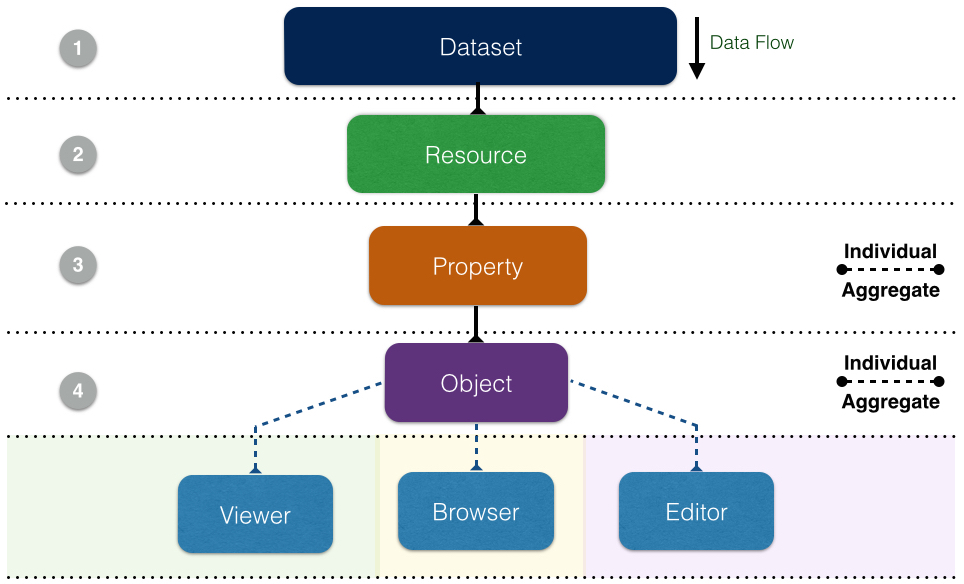
\includegraphics[width=1\linewidth]{images/architecture.jpg}
  \caption{LD-R components architecture.}
  \label{fig:architecture}
\end{figure}

The dataflow in the application starts from the \emph{Dataset} component which handles all the events related to a set of resources under a named graph identified using a URI.
The next level is the \emph{Resource} component which is identified by a URI and indicates what is described in the application.
A resource is specified by a set of properties which are handled by the \emph{Property} component. 
Properties can be either individual or aggregate when combining multiple features of a resource (e.g. a component that combines longitude and latitude properties; start data and end date properties for a date range, etc.).
Each property is instantiated by an individual value or mutiple values in case of an aggreagte object. 
The value(s) of properties are controled by the \emph{Value} component.
Value component invokes different components to view, edit and browse the property values.
\emph{Viewer}, \emph{Editor} and \emph{Browser} components are terminals in the LD-R single directional data flow where customized user-generated components can be plugged into the system.
These components apply on individual and aggregate values (e.g. to show multiple coordinates on a the map).

\begin{figure}[tb]
  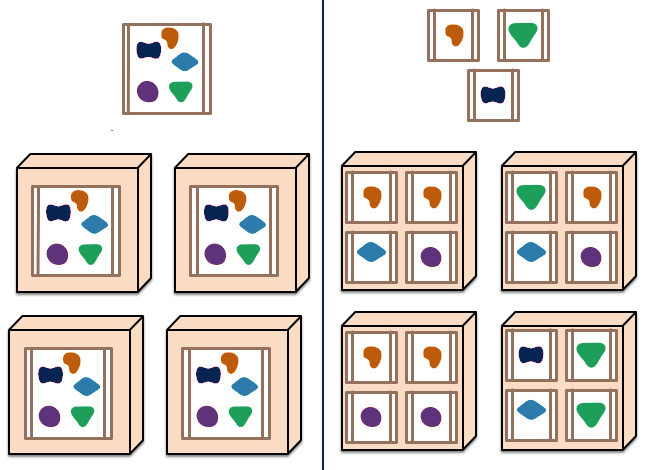
\includegraphics[width=.8\linewidth]{images/microservices.jpg}
  \caption{Monoliths vs. Microservices~\cite{microservices}}
  \label{fig:microservices}
\end{figure}

In contrast to the centalized monolithic architecture, LD-R components comply with \emph{Microservices Architecture}~\cite{microservices}.
As shown in \autoref{fig:microservices}, microservices architecture puts the main functionalities of a component into separete services (instead of in-memory function calls) and scales by distributing these services across servers, replicating as needed.
This architectural style minimizes the redeploying of the entire application when changes in components occur.


%\cite{SmartComposition2015}

\subsection{Scopes and Configurations}

\begin{figure}[tb]
  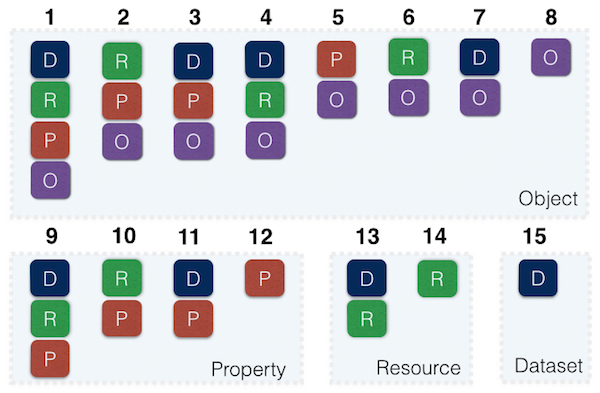
\includegraphics[width=.9\linewidth]{images/scopes.jpg}
  \caption{LD-R scopes based on the permutation of dataset, resource, property and value identifiers.}
  \label{fig:scopes}
\end{figure}

LD-R Web components provide a versatile approach for context adaptation.
A context can be a specific domain of interest, a specific user requirment or both.
In order to enable customization and personalization, LD-R approach exploits the concept of \emph{Scope}.
A scope is defiened as a hierarchical permutation of Dataset, Resource, Property and Value components (cf. \autoref{fig:scopes}).
Each scope conveys a certain level of specificity on a given context ranging from 1 (most specific) to 15 (least specfic).
Scopes are defined by using either the URIs of named graphs, resources and properties; or by identifying the resource types and data types.
UI adaptation is handled by traversing the configs for scopes and overwriting the configs when a more specific scope is found.
For example, on the property level, we can define a generic configuration for all properties and then for some specific properties (e.g. \texttt{dcterms:title} or \texttt{rdfs:label}) within a specific resource (e.g. \texttt{<http://ld-r.org>}), we can change those configurations using the \texttt{RP} scope.
Another example would be having a different rendering for all resources of a specific type (e.g. \texttt{foaf:Person}).

Scopes can also be defined under a specific user which facilitates versioning and reuse of user-specific configs.
User-specifc configs provide different views on components and thereby data, based on the different personas dealing with those components and data.

In addition to the fine-grained component customization, LD-R Web applications provide a fine-grained access control over the data provided by the components.
RDF-based access control in LD-R applications operates at four different granularities provided by the Dataset, Resource, Property and Value component levels and scopes.
For example, application developer can restrict access to a specific property of a specific resource in a certain dataset.

\subsection{Semantic Markup for Web Components}
\label{sec:markup}
Innate support of RDF in LD-R Web components enable the automatic creation of semantic markup in the UI level.
Lower semantic techniques such as RDFa, Mircodata and JSON-LD can be incorporated in an LD-R component to expose structured data to current search engines which are capable of parsing semantic markup.
For example, an LD-R component created based on the Good Relations~\footnote{\url{http://www.heppnetz.de/projects/goodrelations/}} or \url{Schema.org} ontology, can automatically expose the product data as a Google Rich Snippets for products~\footnote{\url{https://developers.google.com/structured-data/}} which will provide better visibility of the data on Web search results (i.e. SEO).

In addition to automatic annotation of data provided by the LD-R Web components, LD-R approach offers semi-automatic markup of Web components by creating component metadata. 
Component metadata consists of two categories of markup:
\begin{itemize}
\item Automatic markup generated by parsing component package specification -- metadata about the component and its dependencies. It inlcudes general metadata such as name, description, version, homepage, author as well as technical metadata on component source repository and dependencies.

\item Manual markup created by component authors which addresses metadata such as component level (dataset, resource, property, value), granularity (individual, aggregate), mode (view, edit, browse) and config parameters specification.

\end{itemize}

Similar to content markup, Component markup can utilize commonly-known ontologies such as \url{Schema.org} in order to provide better visibility and understandability of LD-R components for application assemblers.

\subsection{Stackeholders and Life Cycle}
\begin{figure}[tb]
  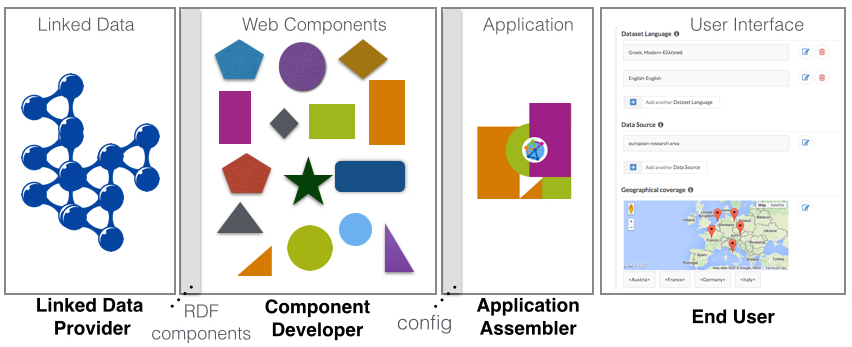
\includegraphics[width=1\linewidth]{images/lifecycle.jpg}
  \caption{LD-R components life cycle.}
  \label{fig:lifecycle}
\end{figure}

As shown in \autoref{fig:lifecycle}, the LD-R components lifecycle encompasses four primary types of stakeholders:

\begin{itemize}

\item \emph{Linked Data Provider}.
Since the LD-R approach focuses mainly on Linked Data applications, provision of RDF-compliant data is an essential phase in developing the LD-R components.
There are different stages~\cite{AuerLOD2} in Linked Data provision such as data extraction, storage, interlinking, enrichment, quality analysis and repair which should be taken into account by data scientists and Linked Data experts.
Once the data and schemata are provided to the LD-R component system, the system can bring a reciprocal value to Linked Data providers to better understand and curate the data when needed.
For example, in case of geo-coordinates, by looking at a map component, data provider can easily curate the outlier data (e.g. ambigious entities) within a certain geo boundary.

\item \emph{Component Developer}. 
It includes UX designers and Web programmers who are involved in component fabrication.
There are two types of Web components developed in this step:
a) \emph{Core components} (cf. \autoref{fig:architecture}) which abstract the underlying RDF data model.
These components are built-in to the system, however can still be overwritten by developers who have profficiency in Semantic Web and Linked Data.
b) \emph{Community-driven components} which exploit the core components.
These components are either created from the scratch or by remixing and repurposing existing Web components found on the Web.

\item \emph{Application Assembler}.
The main task of application assembler is to identify the right components and configurations for the application; and to combine them in a way which fits the application requirement. 
Within the LD-R component system, the metadata provided by each Web component faciliates the discovery of relavant components.
Having shared vocabularies on Linked Open Data allows assemblers to not only reuse components but also reuse the existing configurations and scopes published on the Web.
For example, if there is already a suitable configuration for \texttt{RP} scope which uses \texttt{foaf:Person} as resource type and \texttt{dcterms:description} as property URI, the assembler can reuse that config within his application.

\item \emph{End User}. 
It is the user who experiences working with components to pursue his goals on a certain application domain.
The end user is the one who requests developing a component and the one who sends feedback on the existing components.

\end{itemize}


\section{Implementation}

In order to realize the idea of adaptive Linked Data-driven Web components, we implemented an open-source software framework called \emph{Linked Data Reactor (LD-R)} which is available online at \url{http://ld-r.org}.
LD-R utilizes Facebook's ReactJS\footnote{\url{https://facebook.github.io/react/}} components, Flux\footnote{\url{https://facebook.github.io/flux}} architecture, Yahoo!'s Fluxible\footnote{\url{http://fluxible.io/}} framework for isomorphic Web applications and Semantic-UI\footnote{\url{http://semantic-ui.com/}} framework for flexible UI themes.
The main reasons we chose \emph{React} components over other existing Web Components solutions (e.g. Polymer\footnote{\url{http://www.polymer-project.org/}}, AngularJS\footnote{\url{https://angularjs.org/}}, EmberJS\footnote{\url{http://emberjs.com/}}, etc.) were the maturity of the technology, maintainablity, number of developer tools/components/applications, and efficiency of its underlying virtual DOM approach~\footnote{Elaborating on all these factors is beyond the scope of this paper.}

\begin{figure}[tb]
  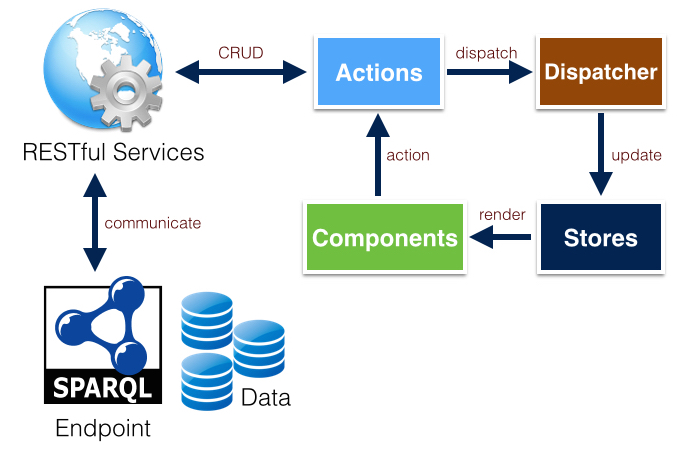
\includegraphics[width=.9\linewidth]{images/dataflow.jpg}
  \caption{Data flow in the LD-R framework.}
  \label{fig:dataflow}
\end{figure}

As shown in \autoref{fig:dataflow}, LD-R follows the Flux architecture which eschews MVC (Model-View-Controller) in favor of a unidirectional data flow. 
When a user interacts with a React component, the component propagates an action through a central dispatcher, to the various stores that hold the application's data and business logic, which updates all of the components that are affected. 
The component interaction with SPARQL endpoints to retrieve and update Linked Data occurs via invoking RESTful services in actions.

In order to allow bootstrapping of LDA UIs, LD-R provides a comprehensive framework that combines the following main elements:
\begin{itemize}

\item A set of RESTful Web services that allow basic CRUD operations on Linked Data by  employing SPARQL queries~\footnote{the framework is compliant with SPARQL 1.1 standard. However, we noticed some incompatibility between Sesame and Virtuoso triple stores. thereby had to implement separate adaptors for them!}.

\item A set of core components called \emph{Reactors} which implement core Linked Data components (see \autoref{fig:architecture}) together with their corresponding actions and stores.

\item A set of default components which allow basic viewing, editing and browsing of Linked Data.

\item A set of minimal viable configurations based on the type of data and properties from commonly-used vocabularies on the Semantic Web (e.g. foaf, dcterms and SKOS).

\item A baisc access control plugin which allows restricting read/write access to data.

\end{itemize}


Semantic markup of data as discussed in Section \ref{sec:markup} is supported natively within the framework by embedding Microdata annotations within LD-R Web components.
Additionally, in order to facilitate creation of components metadata, we developed a tool \footnote{\url{https://github.com/ali1k/ld-r-metadata-generator}} which automatically generates the general metadata about the components in the JSON-LD format using \url{Schema.org} SoftwareApplication schema~\footnote{\url{https://schema.org/SoftwareApplication}}.

\begin{figure*}[ht] 
  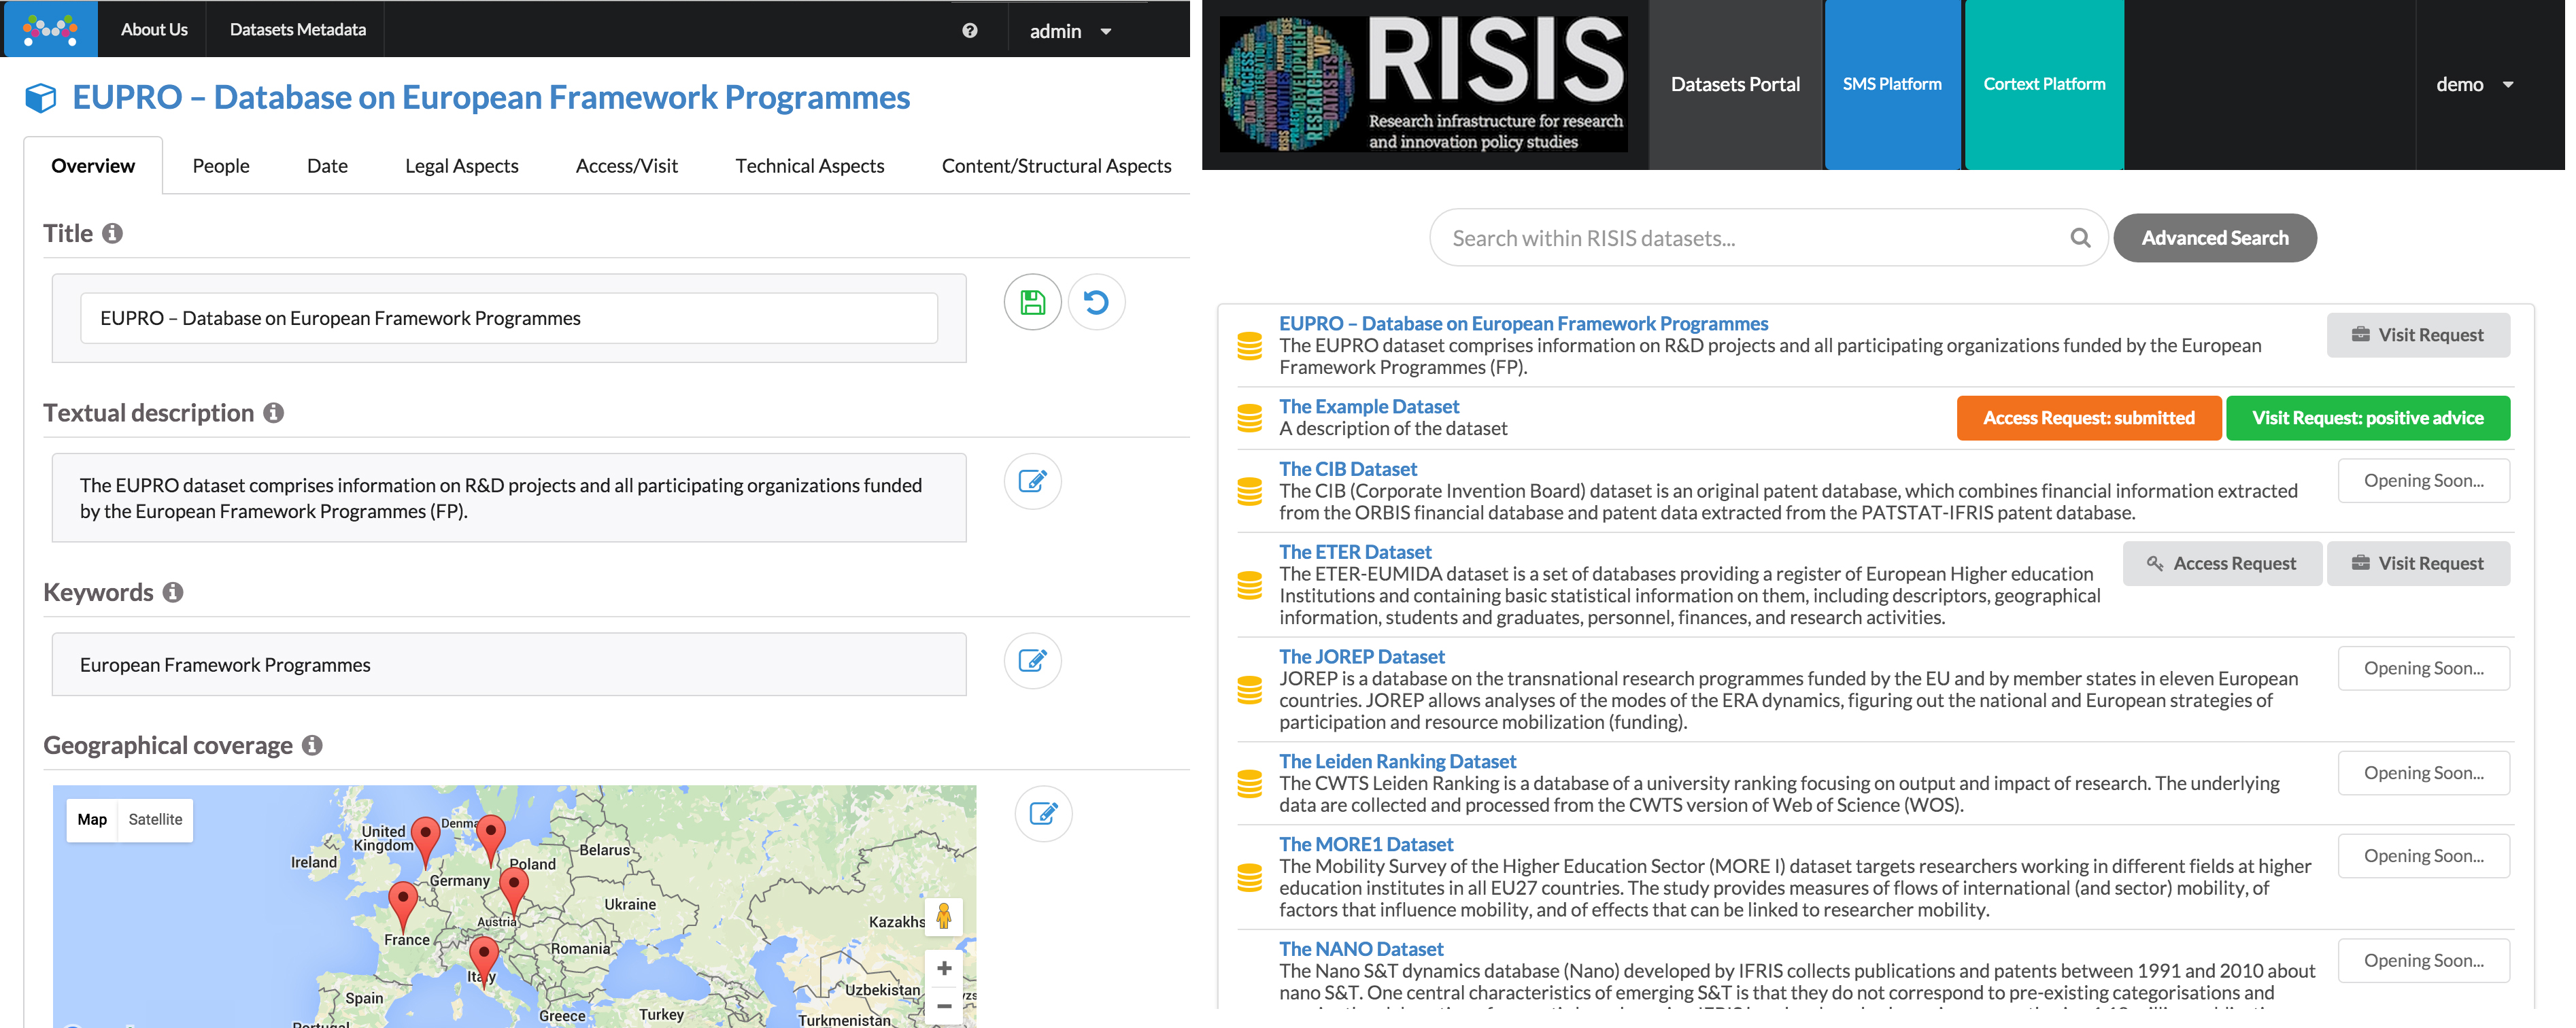
\includegraphics[width=1\linewidth]{images/screenshots.jpg}
  \caption{An screenshot of RISIS metadata editor and datasets portal powered by the LD-R framework.}
\end{figure*}

\section{Use Cases}

LD-R framewok is already in use within the RISIS~\footnote{\url{http://risis.eu}} and OpenPhacts~\footnote{\url{http://www.openphacts.org}} projects.

RISIS project with the aim of providing an infrastructure for research and innovation, targets researchers from various science and technology domains.
LD-R approach was utilized in RISIS to help non-Linked Data experts to provide RDF-based metadata about their datasets~\footnote{\url{http://sms.risis.eu}} and then allowing researchers to search and request data based on the generated metadata~\footnote{\url{http://datasets.risis.eu}}.
In order to expose a user-friendly interface to researchers, the following main configurations and components were required:

\paragraph{Configurations}
\begin{compactitem}
 \item The UI should be able to to render metadata properties in different categories.
 \item The labels for properties should be changeable in the UI esp. in case of technical properties (e.g. RDF dump) unknown to researchers.
 \item There should be a hint for properties to help metadata editors to understand the meaning of the property.
 \item Instead of showing the full URIs, the UI should render either a shortened URI or a meaningful string linked to the original URI. 
 \item When a DBpedia URI is provided, use the Wikipedia URI of the resource in the UI.
 \item If a dropdown menu is provided, there should be the ability to accommoodate user-defined values which are not listed in the menu.
 
\end{compactitem}

\paragraph{Components}
\begin{compactitem}
 \item A component for \texttt{dcterms:spatial} values to allow searching and inserting resources from DBpedia based on the entity type (e.g. Place, Person, Organization, etc).
 \item A component for \texttt{dcterms:subject} values to allow inserting and viewing DBpedia URIs as subject.
 \item A component for \texttt{dcterms:language} values to allow inserting and viewing languages formatted in ISO 639-1 using standard URIs (e.g. \url{http://id.loc.gov/vocabulary/iso639-1/en}).
 \item A component for \texttt{dcat:byteSize} values to allow inserting and viewing file size specified by a unit.
  \item A component for \texttt{dcterms:format} values to allow inserting and viewing mime types.
\end{compactitem}

\begin{lstlisting}[language=json,firstnumber=1, caption=An excerpt of LD-R config for RISIS]
resource: {
    'generic': {
        usePropertyCategories: 1,
        propertyCategories: ['overview', 'people', 'date', 'legalAspects', 'technicalAspects', 'structuralAspects'],
        resourceReactor: ['Resource'],
        shortenURI: 1
    }
},
property: {
    'generic': {
        propertyReactor: ['IndividualProperty'],
        objectReactor: ['IndividualObject'],
        objectIViewer: ['BasicIndividualView'],
        objectIEditor: ['BasicIndividualInput']
    },
    'http://purl.org/dc/terms/language': {
        allowNewValue: 1,
        label: ['Dataset Language'],
        category: ['overview'],
        hint: ['The language of the dataset. Resources defined by the Library of Congress (http://id.loc.gov/vocabulary/iso639-1.html, http://id.loc.gov/vocabulary/iso639-2.html) SHOULD be used.'],
        objectIViewer: ['LanguageView'],
        objectIEditor: ['LanguageInput'],
        defaultValue: ['http://id.loc.gov/vocabulary/iso639-1/en']
    },
    'http://purl.org/dc/terms/spatial': {
         label: ['Geographical coverage'],
         category: ['overview'],
         hint: ['The geographical area covered by the dataset.'],
         allowNewValue: 1,
         objectReactor: ['AggregateObject'],
         objectAViewer: ['DBpediaGoogleMapView'],
         objectIViewer: ['BasicDBpediaView'],
         asWikipedia: 1,
         objectAEditor: ['BasicAggregateInput'],
         objectIEditor: ['DBpediaInput'],
         lookupClass: ['Place']
     },
    'http://purl.org/dc/terms/subject': {
        category: ['overview'],
        label: ['Keywords'],
        hint: ['Tags a dataset with a topic.'],
        allowNewValue: 1,
        objectIEditor: ['DBpediaInput'],
        objectIViewer: ['BasicDBpediaView'],
        asWikipedia: 1
    }    
}
\end{lstlisting}

\section{Discussion}

\section{Related Work}

Web Components and the Semantic Web~\cite{pahl2011}

Semantic Web Services

Existing tools to view/edit and browse LD e.g. OntoWiki, Saha


\section{Conclusion}

Future work: UI for generating configs

\section{Aknowledgement}
We would like to thank our colleagues from the KRR research group at VU University Amsterdam for their helpful comments during the development of the LD-R framework. This work was supported by a grant from the European Union's 7th Framework Programme provided for the project RISIS (GA no. 313082).


\bibliographystyle{abbrv}
\bibliography{refs}

\end{document}
